%% For double-blind review submission, w/o CCS and ACM Reference (max submission space)
\documentclass[sigplan,10pt,review,anonymous]{acmart}
\settopmatter{printfolios=true,printccs=false,printacmref=false}
%% For double-blind review submission, w/ CCS and ACM Reference
%\documentclass[sigplan,review,anonymous]{acmart}\settopmatter{printfolios=true}
%% For single-blind review submission, w/o CCS and ACM Reference (max submission space)
%\documentclass[sigplan,review]{acmart}\settopmatter{printfolios=true,printccs=false,printacmref=false}
%% For single-blind review submission, w/ CCS and ACM Reference
%\documentclass[sigplan,review]{acmart}\settopmatter{printfolios=true}
%% For final camera-ready submission, w/ required CCS and ACM Reference
%\documentclass[sigplan]{acmart}\settopmatter{}


%% Conference information
%% Supplied to authors by publisher for camera-ready submission;
%% use defaults for review submission.
%\acmConference[ARRAY'22]{ACM SIGPLAN Conference on Programming Languages}{June 13, 2022}{San Diego, CA, USA}
%\acmYear{2018}
%\acmISBN{} % \acmISBN{978-x-xxxx-xxxx-x/YY/MM}
%\acmDOI{} % \acmDOI{10.1145/nnnnnnn.nnnnnnn}
%\startPage{1}

%% Copyright information
%% Supplied to authors (based on authors' rights management selection;
%% see authors.acm.org) by publisher for camera-ready submission;
%% use 'none' for review submission.
\setcopyright{none}
%\setcopyright{acmcopyright}
%\setcopyright{acmlicensed}
%\setcopyright{rightsretained}
%\copyrightyear{2018}           %% If different from \acmYear

\usepackage{dsfont}
\usepackage{stmaryrd}
\usepackage{colortbl}

%% Bibliography style
\bibliographystyle{acmart}

\usepackage{dsfont}
\usepackage{stmaryrd}
\usepackage{colortbl}
\usepackage{hyperref}

\usepackage{amsmath}
\DeclareMathOperator*{\argmax}{argmax}
\DeclareMathOperator*{\argmin}{argmin}
\usepackage{amssymb}

\usepackage[dvipsnames, table]{xcolor}
\usepackage{textcomp}

% Packages
\usepackage[pdf]{graphviz}
\usepackage{mathrsfs}

\newcommand*\circled[1]{\tikz[baseline=-0.1cm]{
  \node[shape=circle,draw,inner sep=0.48pt] (char) {\fontsize{7}{12}\textsf{#1}};}}

\DeclareMathAlphabet{\mathcal}{OMS}{cmsy}{m}{n}
\usepackage{cancel}
\newcommand\ccancel[2][red]{\renewcommand\CancelColor{\color{#1}}\cancel{#2}}
\newcommand{\nDownarrow}{\ensuremath{\text{ }\cancel{\Downarrow}\text{ }}}
\usepackage{centernot}

\usepackage{pgfplots, pgfplotstable}
\pgfplotsset{compat=1.7}
\usepgfplotslibrary{fillbetween}
\usetikzlibrary{patterns}
\pgfmathdeclarefunction{gauss}{2}{\pgfmathparse{1/(#2*sqrt(2*pi))*exp(-((x-#1)^2)/(2*#2^2))}}
\pgfmathdeclarefunction{nil}{1}{\pgfmathparse{0.001}}

\usepackage{arydshln}
\usepackage{adjustbox}
\usepackage{enumerate}
\usepackage{enumitem}
\usepackage{tikz-cd}
\usetikzlibrary{calc}
\usepackage{amsfonts}
%\usepackage{prooftrees}
\usepackage{bussproofs}
\renewcommand{\sectionautorefname}{\S}
\renewcommand{\subsectionautorefname}{\S}
\usepackage{float}

\usepackage{tikz-3dplot}
\usetikzlibrary{3d}
\usetikzlibrary{calligraphy}
\newif\ifshowcellnumber
\showcellnumbertrue

\usepackage{algorithm}
\usepackage{algpseudocode}
\usepackage{algorithmicx}
\usepackage{sourcecodepro}
\usepackage{tikz-qtree}
\usepackage{amsthm}
\usepackage{bm}
\usetikzlibrary{bayesnet}
\usetikzlibrary{arrows}
\usepackage{subcaption}
\usetikzlibrary{backgrounds}
\usetikzlibrary{tikzmark}
\usetikzlibrary{hobby}

\usepackage{mwe}

\newcommand{\E}{\mathbb{E}}
\newcommand{\Var}{\mathrm{Var}}
\newcommand{\Cov}{\mathrm{Cov}}

\newcommand{\CompOrder}{\mathcal{O}}
\def\graphspace{\mathbf{G}}
\def\Uniform{\mbox{\rm Uniform}}
\def\Gaussian{\mbox{\rm Gaussian}}
\def\Bernoulli{\mbox{\rm Bernoulli}}
\def\Dirichlet{\mbox{\rm Dirichlet}}

\usepackage{mathtools}% superior to amsmath
\usepackage{tikz}
% Packages
\usepackage{listings}
\DeclareRobustCommand{\hlred}[1]{{\sethlcolor{pink}\hl{#1}}}
\usepackage{fontspec}

\setmonofont[Scale=0.8]{JetBrainsMono}[
  Contextuals={Alternate},
  Path=./font/,
  Extension = .ttf,
  UprightFont=*-Regular,
  BoldFont=*-Bold,
  ItalicFont=*-Italic,
  BoldItalicFont=*-BoldItalic
]

\usepackage[skins,breakable,listings]{tcolorbox}

\lstdefinelanguage{kotlin}{
  comment=[l]{//},
  commentstyle={\color{gray}\ttfamily},
  emph={delegate, filter, firstOrNull, forEach, it, lazy, mapNotNull, println, repeat, assert, with, head, tail, len, return@},
  numberstyle=\noncopyable,
  identifierstyle=\color{black},
  keywords={abstract, actual, as, as?, break, by, class, companion, continue, data, do, dynamic, else, enum, expect, false, final, for, fun, get, if, import, in, infix, interface, internal, is, null, object, open, operator, override, package, private, public, return, sealed, set, super, suspend, this, throw, true, try, catch, typealias, val, var, vararg, when, where, while, tailrec, reified},
  keywordstyle={\bfseries},
  morecomment=[s]{/*}{*/},
  morestring=[b]",
  morestring=[s]{"""*}{*"""},
  ndkeywords={@Deprecated, @JvmField, @JvmName, @JvmOverloads, @JvmStatic, @JvmSynthetic, Array, Byte, Double, Float, Boolean, Int, Integer, Iterable, Long, Runnable, Short, String, int},
  ndkeywordstyle={\bfseries},
  sensitive=true,
  stringstyle={\ttfamily},
  literate={`}{{\char0}}1,
  escapeinside={(*@}{@*)}
}
\lstdefinelanguage{tidy}{
  comment=[l]{//},
  commentstyle={\color{gray}\ttfamily},
  emph={|, ->, ---},
  emphstyle={\color{red}},
  identifierstyle=\color{black},
  keywords={\|, ->, ---},
  otherkeywords={|,->},
  morekeywords={|,->},
  keywordstyle={\color{blue}\bfseries},
  morecomment=[s]{/*}{*/},
  morestring=[b]",
  morestring=[s]{"""*}{*"""},
  ndkeywords={@Deprecated, @JvmField, @JvmName, @JvmOverloads, @JvmStatic, @JvmSynthetic, Array, Byte, Double, Float, Int, Integer, Iterable, Long, Runnable, Short, String},
  ndkeywordstyle={\color{orange}\bfseries},
  sensitive=true,
  stringstyle={\color{green}\ttfamily},
  literate={`}{{\char0}}1
}

%%%%%%%%%%%%%%%%%%%%%%%%%%%%%%%%%%%%%%%%%%%
%
% Color boxes
%
%%%%%%%%%%%%%%%%%%%%%%%%%%%%%%%%%%%%%%%%%%%

\tcbset{
  enhanced jigsaw,
  breakable,
  listing only,
%  boxsep=-1pt,
%  top=-1pt,
  bottom=0.1cm,
  right=0.5cm,
  overlay first={
    \node[black!50] (S) at (frame.south) {\Large\ding{34}};
    \draw[dashed,black!50] (frame.south west) -- (S) -- (frame.south east);
  },
  overlay middle={
    \node[black!50] (S) at (frame.south) {\Large\ding{34}};
    \draw[dashed,black!50] (frame.south west) -- (S) -- (frame.south east);
    \node[black!50] (S) at (frame.north) {\Large\ding{34}};
    \draw[dashed,black!50] (frame.north west) -- (S) -- (frame.north east);
  },
  overlay last={
    \node[black!50] (S) at (frame.north) {\Large\ding{34}};
    \draw[dashed,black!50] (frame.north west) -- (S) -- (frame.north east);
  },
  before={\par\vspace{5pt}},
  after={\par\vspace{\parskip}\noindent}
}

\definecolor{slightgray}{rgb}{0.90, 0.90, 0.90}

\usepackage{soul}
\makeatletter
\def\SOUL@hlpreamble{%
  \setul{}{3.0ex}%
  \let\SOUL@stcolor\SOUL@hlcolor%
  \SOUL@stpreamble%
}
\makeatother

\newcommand{\inline}[1]{%
  \begingroup%
  \sethlcolor{slightgray}%
  \hl{\ttfamily\footnotesize #1}%
  \endgroup
}

\newcommand{\tinline}[1]{%
  \begingroup%
  \sethlcolor{slightgray}%
  \hl{\ttfamily\tiny #1}%
  \endgroup
}

\newtcblisting{halftidyinput}[1][]{%
  left skip=0.7cm,
  left=0.35cm,
  width=6cm,
%  left=-0.01cm,
  top=-0.1cm,
  bottom=-0.35cm,
  listing options={
    language=tidy,
    basicstyle=\ttfamily\small,
%numberstyle=\footnotesize,
    showstringspaces=false,
    tabsize=2,
    breaklines=true,
    numbers=none,
    inputencoding=utf8,
    escapeinside={(*@}{@*)},
    #1
  },
  underlay unbroken and first={%
    \path[draw=none] (interior.north west) rectangle node[white]{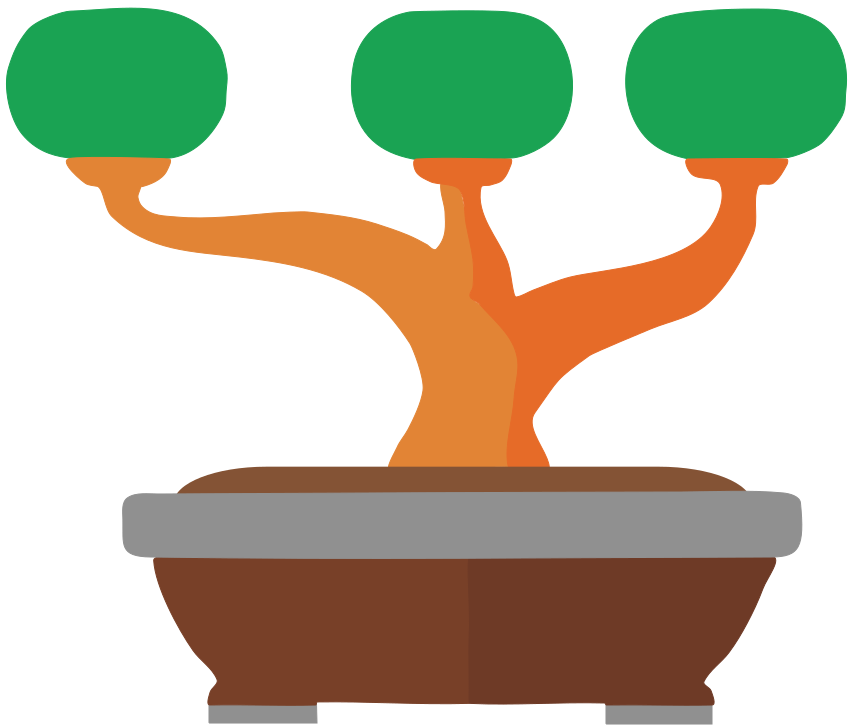
\includegraphics[width=4mm]{../figures/tidyparse_logo.png}} ([xshift=-10mm,yshift=-7mm]interior.north west);
  }
}

\newtcblisting{wholetidyinput}[1][]{%
  left skip=0.7cm,
  left=0.35cm,
  top=0.1cm,
  middle=0mm,
  boxsep=0mm,
  listing options={
    language=tidy,
    basicstyle=\ttfamily\small,
%numberstyle=\footnotesize,
    showstringspaces=false,
    tabsize=2,
    breaklines=true,
    numbers=none,
    inputencoding=utf8,
    escapeinside={(*@}{@*)},
    #1
  },
  underlay unbroken and first={%
      \path[draw=none] (interior.north west) rectangle node[white]{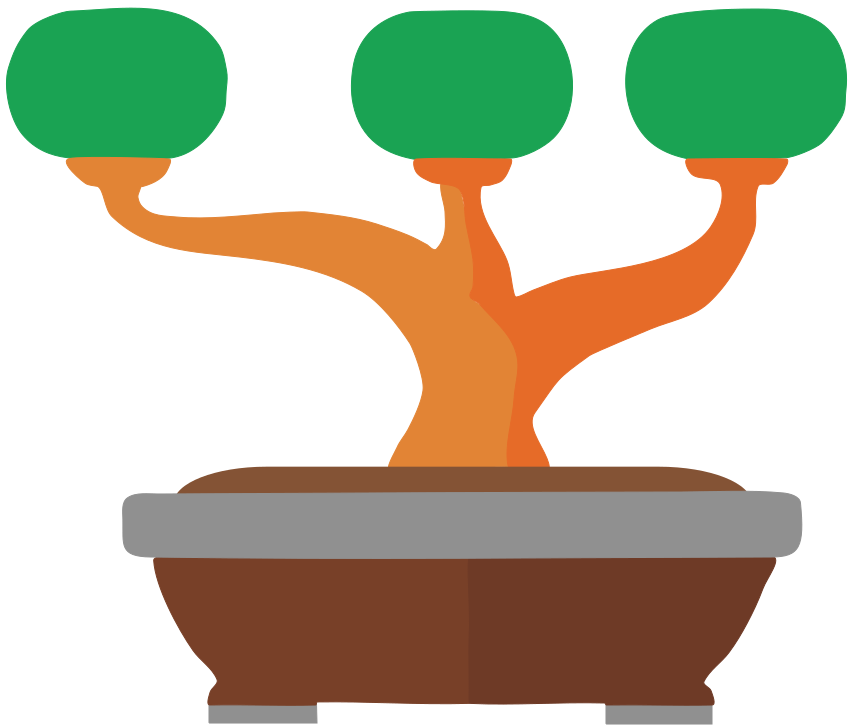
\includegraphics[width=4mm]{../figures/tidyparse_logo.png}} ([xshift=-10mm,yshift=-9mm]interior.north west);
  }
}

\definecolor{A}{RGB}{6,150,104}
\definecolor{B}{RGB}{196,74,137}
\definecolor{C}{RGB}{117,237,133}
\definecolor{D}{RGB}{246,46,243}
\definecolor{E}{RGB}{89,162,12}
\definecolor{F}{RGB}{113,12,158}
\definecolor{G}{RGB}{191,205,142}
\definecolor{H}{RGB}{51,58,158}
\definecolor{I}{RGB}{244,212,3}
\definecolor{J}{RGB}{37,36,249}
\definecolor{K}{RGB}{253,165,71}
\definecolor{L}{RGB}{27,81,29}
\colorlet{LA}{A!30}
\colorlet{LB}{B!30}
\colorlet{LC}{C!30}
\colorlet{LD}{D!30}
\colorlet{LE}{E!30}
\colorlet{LF}{F!30}
\colorlet{LG}{G!30}
\colorlet{LH}{H!30}
\colorlet{LI}{I!30}
\colorlet{LJ}{J!30}
\colorlet{LK}{K!30}
\colorlet{LL}{L!30}
\newcommand{\hiliA}[1]{%
  \colorbox{LA}{$#1$}}
\newcommand{\hiliB}[1]{%
  \colorbox{LB}{$#1$}}
\newcommand{\hiliC}[1]{%
  \colorbox{LC}{$#1$}}
\newcommand{\hiliD}[1]{%
  \colorbox{LD}{$#1$}}
\newcommand{\hiliE}[1]{%
  \colorbox{LE}{$#1$}}
\newcommand{\hiliF}[1]{%
  \colorbox{LF}{$#1$}}
\newcommand{\hiliG}[1]{%
  \colorbox{LG}{$#1$}}
\newcommand{\hiliH}[1]{%
  \colorbox{LH}{$#1$}}
\newcommand{\hiliI}[1]{%
  \colorbox{LI}{$#1$}}
\newcommand{\hiliJ}[1]{%
  \colorbox{LJ}{$#1$}}
\newcommand{\hiliK}[1]{%
  \colorbox{LK}{$#1$}}
\newcommand{\hiliL}[1]{%
  \colorbox{LL}{$#1$}}
\newcommand{\highlight}[1]{%
  \colorbox{lgray}{$#1$}}
\colorlet{lred}{red!30}
\colorlet{lorange}{orange!30}
\colorlet{lgreen}{green!30}
\colorlet{lgray}{black!15}
\colorlet{dgray}{black!75}
\DeclareRobustCommand{\hlred}[1]{{\sethlcolor{lred}\hl{#1}}}
\DeclareRobustCommand{\hlorange}[1]{{\sethlcolor{lorange}\hl{#1}}}
\DeclareRobustCommand{\hlgreen}[1]{{\sethlcolor{lgreen}\hl{#1}}}
\DeclareRobustCommand{\hlgray}[1]{{\sethlcolor{lgray}\hl{#1}}}
\DeclareRobustCommand{\caret}[1]{{\sethlcolor{dgray}\textcolor{white}{\hl{#1}}}}

\usepackage{url}
\usepackage{qtree}

\usepackage{filecontents}
\usepackage{pstricks-add}
\usepackage{emoji}
\usepackage{alltt}
\usepackage{nicematrix}
\usepackage{graphicx}
\usepackage{ulem}
\usepackage{upquote}
\tikzstyle{every picture}+=[remember picture]
\usepackage{menukeys}
\pgfplotstableread[col sep=comma,]{timings_loc.csv}\loctimings
\pgfplotstableread[col sep=comma,]{timings_unloc.csv}\unloctimings

\makeatletter
\DeclareRobustCommand{\cev}[1]{%
  {\mathpalette\do@cev{#1}}%
}
\newcommand{\do@cev}[2]{%
  \vbox{\offinterlineskip
  \sbox\z@{$\m@th#1 x$}%
  \ialign{##\cr
  \hidewidth\reflectbox{$\m@th#1\vec{}\mkern4mu$}\hidewidth\cr
  \noalign{\kern-\ht\z@}
    $\m@th#1#2$\cr
  }%
  }%
}
\makeatother

\makeatletter
\DeclareRobustCommand{\pder}[1]{%
  \@ifnextchar\bgroup{\@pder{#1}}{\@pder{}{#1}}}
\newcommand{\@pder}[2]{\frac{\partial#1}{\partial#2}}
\makeatother

\newcommand{\shup}{\shortuparrow}
\newcommand{\shri}{\shortrightarrow}
\newcommand{\shur}{\shup\hspace{-5pt}\shri}

\makeatletter
\def\squigglyred{\bgroup \markoverwith{\textcolor{red}{\lower3\p@\hbox{\sixly \char58}}}\ULon}
\makeatother

\makeatletter
\def\squigglyblu{\bgroup \markoverwith{\textcolor{blue}{\lower3\p@\hbox{\sixly \char58}}}\ULon}
\makeatother

\makeatletter
\def\squigglyora{\bgroup \markoverwith{\textcolor{orange}{\lower3\p@\hbox{\sixly \char58}}}\ULon}
\makeatother

\newcommand{\err}[1]{\smash{\squigglyred{#1}{}}}
\newcommand{\erb}[1]{\smash{\squigglyblu{#1}{}}}
\newcommand{\ero}[1]{\smash{\squigglyora{#1}{}}}
\newcommand{\stirlingii}{\genfrac{\{}{\}}{0pt}{}}

%======== Arrows =========
\newcommand{\knightarrow}{
  \tikz{
    \fill (0pt,0pt) circle [radius = 1pt];
    \fill (0pt,6pt) circle [radius = 1pt];
    \fill (6pt,0pt) circle [radius = 1pt];
    \fill (6pt,6pt) circle [radius = 1pt];
    \fill (12pt,0pt) circle [radius = 1pt];
    \fill (12pt,6pt) circle [radius = 1pt];
    \fill (6pt,0pt) circle [radius = 1pt];
    \fill (12pt,0pt) circle [radius = 1pt];
    \draw [-to] (0pt,0pt) -- (12pt,6pt);
  }
}

\newcommand{\kingarrow}{
  \tikz{
    \fill (0pt,0pt) circle [radius = 1pt];
    \fill (6pt,0pt) circle [radius = 1pt];
    \fill (0pt,6pt) circle [radius = 1pt];
    \fill (6pt,6pt) circle [radius = 1pt];
    \draw [-to] (0pt,0pt) -- (6pt,6pt);
    \draw [-to] (0pt,0pt) -- (0pt,6pt);
    \draw [-to] (0pt,0pt) -- (6pt,0pt);
  }
}

\newcommand{\duparrow}{
  \tikz{
    \fill (0pt,0pt) circle [radius = 1pt];
    \fill (0pt,6pt) circle [radius = 1pt];
    \draw [-to] (0pt,0pt) -- (0pt,6pt);
  }
}

\newcommand{\drightarrow}{
  \tikz{
    \fill (0pt,0pt) circle [radius = 1pt];
    \fill (6pt,0pt) circle [radius = 1pt];
    \draw [-to] (0pt,0pt) -- (6pt,0pt);
  }
}

\newcommand{\ddiagarrow}{
  \tikz{
    \fill (0pt,0pt) circle [radius = 1pt];
    \fill (6pt,0pt) circle [radius = 1pt];
    \fill (0pt,6pt) circle [radius = 1pt];
    \fill (6pt,6pt) circle [radius = 1pt];
    \draw [-to] (0pt,0pt) -- (6pt,6pt);
  }
}

\newcommand{\knightkingarrow}{
  \tikz{
    \fill (0pt,0pt) circle [radius = 1pt];
    \fill (0pt,6pt) circle [radius = 1pt];
    \fill (6pt,0pt) circle [radius = 1pt];
    \fill (6pt,6pt) circle [radius = 1pt];
    \fill (12pt,0pt) circle [radius = 1pt];
    \fill (12pt,6pt) circle [radius = 1pt];
    \draw [-to] (0pt,0pt) -- (6pt,6pt);
    \draw [-to] (0pt,0pt) -- (0pt,6pt);
    \draw [-to] (0pt,0pt) -- (6pt,0pt);
    \draw [-to] (0pt,0pt) -- (12pt,6pt);
  }
}

%======== Arrows =========

\usetikzlibrary{decorations.pathreplacing,automata,calc,positioning,matrix,fit,decorations.pathmorphing}

\usepackage{wrapfig}

\newcommand{\mkTrellis}[1]{
  \begin{tikzpicture}
    \def\dx{20pt}
    \def\dy{30pt}
    \newcounter{i}
    \stepcounter{i}
    \node[circle, draw, fill=black!30] (\arabic{i}) at (0,0){};
    \foreach [count=\i] \x in {2,...,#1}{
      \pgfmathsetmacro{\lox}{\x-1}%
      \pgfmathsetmacro{\loxt}{\x-3}%
      \foreach [count=\j] \xx in {-\lox,-\loxt,...,\lox}{
        \pgfmathsetmacro{\jj}{\j-1}%
        \stepcounter{i}
        \pgfmathsetmacro{\kk}{\xx-2}%
        \pgfmathsetmacro{\lbl}{\lox!/(\jj!*(\lox-\jj)!)}
        \ifnum\x<\kk
        \pgfmath\node[circle, draw]  (\arabic{i}) at (\xx*\dx, -\lox*\dy) {};
        \else
        \pgfmath\node[circle, draw, fill=black!30]  (\arabic{i}) at (\xx*\dx, -\lox*\dy) {};
        \fi
      }
    }
    \newcounter{z}
    \newcounter{xn}
    \newcounter{xnn}
    \pgfmathsetmacro{\maxx}{#1 - 1}
    \foreach \x in {1,...,\maxx}{
      \foreach \xx in {1,...,\x}{
        \stepcounter{z}
        \setcounter{xn}{\arabic{z}}
        \addtocounter{xn}{\x}
        \setcounter{xnn}{\arabic{xn}}
        \stepcounter{xnn}
        \draw [<-] (\arabic{z}) -- (\arabic{xn});
        \draw [<-] (\arabic{z}) -- (\arabic{xnn});
      }
    }
  \end{tikzpicture}
}

\newcommand{\dx}{20pt}
\newcommand{\dy}{30pt}
\newcounter{i}
\newcounter{z}
\newcounter{xn}
\newcounter{xnn}
\newcommand{\mkTrellisAppend}[1]{
  \begin{tikzpicture}
    \setcounter{i}{0}
    \setcounter{z}{0}
    \setcounter{xn}{0}
    \setcounter{xnn}{0}
    \stepcounter{i}
    \node[circle, draw] (\arabic{i}) at (0,0){};
    \foreach [count=\i] \x in {2,...,#1}{
      \pgfmathsetmacro{\lox}{\x-1}%
      \pgfmathsetmacro{\loxt}{\x-3}%
      \foreach [count=\j] \xx in {-\lox,-\loxt,...,\lox}{
        \pgfmathsetmacro{\jj}{\j-1}%
        \stepcounter{i}
        \pgfmathsetmacro{\kk}{\xx+2}%
        \pgfmathsetmacro{\lbl}{\lox!/(\jj!*(\lox-\jj)!)}
        \ifnum\x>\kk
        \pgfmath\node[circle, draw, fill=black!30]  (\arabic{i}) at (\xx*\dx, -\lox*\dy) {};
        \else
        \pgfmath\node[circle, draw]  (\arabic{i}) at (\xx*\dx, -\lox*\dy) {};
        \fi
      }
    }
    \pgfmathsetmacro{\maxx}{#1 - 1}
    \foreach \x in {1,...,\maxx}{
      \foreach \xx in {1,...,\x}{
        \stepcounter{z}
        \setcounter{xn}{\arabic{z}}
        \addtocounter{xn}{\x}
        \setcounter{xnn}{\arabic{xn}}
        \stepcounter{xnn}
        \draw [<-] (\arabic{z}) -- (\arabic{xn});
        \draw [<-] (\arabic{z}) -- (\arabic{xnn});
      }
    }
  \end{tikzpicture}
}

\newcommand{\mkTrellisInsert}[1]{
  \begin{tikzpicture}
    \setcounter{i}{0}
    \setcounter{z}{0}
    \setcounter{xn}{0}
    \setcounter{xnn}{0}
    \stepcounter{i}
    \node[circle, draw] (\arabic{i}) at (0,0){};
    \foreach [count=\i] \x in {2,...,#1}{
      \pgfmathsetmacro{\lox}{\x-1}%
      \pgfmathsetmacro{\loxt}{\x-3}%
      \foreach [count=\j] \xx in {-\lox,-\loxt,...,\lox}{
        \pgfmathsetmacro{\jj}{\j-1}%
        \stepcounter{i}
        \pgfmathsetmacro{\mp}{\xx+#1}%
        \pgfmathsetmacro{\mq}{\xx+\x}%
        \pgfmathsetmacro{\lbl}{\lox!/(\jj!*(\lox-\jj)!)}
        \ifnum\x>\mp
        \pgfmath\node[circle, draw, fill=black!30]  (\arabic{i}) at (\xx*\dx, -\lox*\dy) {};
        \else
        \ifnum#1<\mq
        \pgfmath\node[circle, draw, fill=black!30]  (\arabic{i}) at (\xx*\dx, -\lox*\dy) {};
        \else
        \pgfmath\node[circle, draw]  (\arabic{i}) at (\xx*\dx, -\lox*\dy) {};
        \fi
        \fi

      }
    }
    \pgfmathsetmacro{\maxx}{#1 - 1}
    \foreach \x in {1,...,\maxx}{
      \foreach \xx in {1,...,\x}{
        \stepcounter{z}
        \setcounter{xn}{\arabic{z}}
        \addtocounter{xn}{\x}
        \setcounter{xnn}{\arabic{xn}}
        \stepcounter{xnn}
        \draw [<-] (\arabic{z}) -- (\arabic{xn});
        \draw [<-] (\arabic{z}) -- (\arabic{xnn});
      }
    }
  \end{tikzpicture}
}

\usetikzlibrary{automata, positioning, arrows}

\newcommand{\nobarfrac}{\genfrac{}{}{0pt}{}}
\pgfplotstableread[col sep=comma,]{timings_loc.csv}\loctimings
\pgfplotstableread[col sep=comma,]{timings_unloc.csv}\unloctimings
\pgfplotstableread[col sep=comma,]{natural_errors.csv}\naturalerrors
\pgfplotstableread[col sep=comma,]{synthetic_errors.csv}\syntheticerrors

\usepackage[all,pdf]{xy}

\newcommand{\bs}{\blacksquare}
\newcommand{\ws}{\square}
\begin{document}

%% Title information
\title{Probabilistic Array Programming on Galois Fields}
\begin{abstract}
We present a framework for probabilistic program synthesis based on Galois theory. This framework is capable of modeling discrete distributions, parsing context free languages, graph representation learning and sketch-based program synthesis, all using sparse matrix multiplication on $GF(p^n)$. This elegant representation allows us to leverage complexity-theoretic lower bounds and easily access various compiler targets, including low level languages like VHDL and netlist as well as higher level IRs such as JVM, LLVM, and JS using the same codebase. We discuss its theory, implementation and a few use cases, which include learning and sketching syntax and simple programs via SAT/SMT encoding.
\end{abstract}
\maketitle

\section{Introduction}

A Galois field is a field containing a finite set of elements, e.g., $\mathbb{Z}/n$ where $n$ is prime. We are primarily interested in GF$(2^n)$, taking values on $\{0, 1\}^n$, due to its amenability to SAT/SMT encoding, well-studied theoretical properties, circuit synthesizability and broad applicability to signal processing and computational linguistics. For example, the theory of context free grammars are a special case~\citep{jansson2016certified, bakinova2020formal}. Given a CFG $\mathcal{G} := \langle V, \Sigma, P, S\rangle$ in Chomsky Normal Form, we can construct a recognizer $R_\mathcal{G}: \Sigma^n \rightarrow \mathbb{B}$ for strings $\sigma: \Sigma^n$ as follows. Let $\mathcal P(V)$ be our domain, $0$ be $\varnothing$, $\oplus$ be $\cup$, and $\otimes$ be defined as:

\vspace{-7pt}
\[
a \otimes b := \{C \mid \langle A, B\rangle \in a \times b, (C\rightarrow AB) \in P\}
\]

\noindent We initialize $\mathbf{M}^0_{r,c}(\mathcal{G}, \sigma) \coloneqq \{V \mid c = r + 1, (V \rightarrow \sigma_r) \in P\}$ and search for a matrix $\mathbf{M}^*$ via fixpoint iteration,

\vspace{-5}
\[
\mathbf{M}^* = \begin{pmatrix}
            \varnothing & \{V\}_{\sigma_1} & \ldots & \ldots & \mathcal{T} \\
            \varnothing & \varnothing & \{V\}_{\sigma_2} & \ldots & \ldots \\
            \varnothing & \varnothing & \varnothing & \{V\}_{\sigma_3} & \ldots \\
            \varnothing & \varnothing & \varnothing & \varnothing & \{V\}_{\sigma_4} \\
            \varnothing & \varnothing & \varnothing & \varnothing & \varnothing
\end{pmatrix}
\]

\noindent where $\mathbf{M}^*$ is the least solution to $\mathbf{M} = \mathbf{M} + \mathbf{M}^2$. We can then define the recognizer as $R \coloneqq \mathds{1}_{\mathcal{T}}(S) \iff \mathds{1}_{\mathcal{L}(\mathcal{G})}(\sigma)$.

This decision procedure can be lowered to binary matrices by noting $\bigoplus_{k = 1}^n \mathbf{M}_{ik} \otimes \mathbf{M}_{kj}$ has cardinality bounded by $|V|$ and is thus representable as a fixed-length vector. Full details of this bisimilarity can be found in Valiant~\citep{valiant1975general} and Lee~\citep{lee2002fast}, who proves its time complexity to be $\mathcal{O}(n^\omega)$ where $\omega$ is the matrix multiplication bound (currently $\omega < 2.763$~\citep{harris2021improved} as of writing this manuscript). Assuming sparsity, this technique can typically be reduced to linearithmic time, and is currently the best asymptotic bound for CFL recognition to date.

\noindent A similar procedure may be used to learn, parse and sample from probabilistic grammars such as PCFGs~\citep{goodman1999semiring} and probabilistic circuits~\citep{peharz2015foundations} using \textit{semirings}, many of which have carrier sets that can be compactly represented as elements of GF$(2^n)$. Known as \textit{propagation} or \textit{message passing}, this procedure consists of two steps: \textit{aggregate} and \textit{update}. Let $\delta_{st}$ denote some distance metric on a path between vertices $s$ and $t$ in a graph. To obtain $\delta_{st}$, one may run the following procedure using a desired path algebra until convergence:\\

\vspace{-7}
  \hspace{-12}\begin{tabular}{lcr}
    $\delta_{st} = \overbrace{\underset{P\in P_{st}^*}{\bigoplus}\underbrace{\underset{e\in P}{\bigotimes}W_{e}}_{\text{Aggregate}}}^{\text{Update}}$ & &
    \bgroup
    \def\arraystretch{1.2}
    \begin{tabular}{c{1cm}c{1cm}|c{1cm}c{1cm}|c}
      $\oplus$ & $\otimes$ & $\circled{0}$ & $\circled{1}$ & Path     \\\hline
      min      & +         &   $\infty$    &      0        & Shortest \\
      max      & +         &   $-\infty$   &      0        & Longest  \\
      max      & min       &       0       &   $\infty$    & Widest   \\
      $\vee$   & $\underline{\vee}$ &  $\circ$   &  $\top$  & Random \\
    \end{tabular}
    \egroup
  \end{tabular}\\

\noindent Many dynamic programming algorithms, including Bellman-Ford, Floyd-Warshall, Dijkstra's shortest path, as well as belief, constraint, error, expectation and backpropagation can be neatly expressed as semiring algebras. We refer the curious reader to Gondran~\citep{gondran2008graphs} and Baras~\citep{baras2010path} for an extensive survey of the algebraic path problem and its many wonderful applications throughout statistics and computer science.

GF$(2^n)$ can also be used to search over highly complex state spaces and sample without replacement from arbitrarily large sets. Let $\textbf{M}: \text{GF}(2^{n\times n})$ be a square matrix defined as $\mathbf{M}^0_{r, c} = P_c \text{ if } r=0 \text{ else } \mathds{1}[c = r - 1]$ where $P$ is a feedback polynomial over $GF(2^n)$ with coefficients $P_{1\ldots n}$ and semiring operators $\otimes := \underline{\vee}, \oplus := \vee$ lifted to matrices in the usual way:

\vspace{-7}
\[
\mathbf{M}^tV = \begin{pmatrix}
  P_0 & P_1 & P_2 & P_3 & P_4 \\
  \top & \circ & \circ & \circ & \circ \\
  \circ & \top & \circ & \circ & \circ \\
  \circ & \circ & \top & \circ & \circ \\
  \circ & \circ & \circ & \top & \circ
\end{pmatrix}^t
\begin{pmatrix}
      V_0 \\
      V_1 \\
      V_2 \\
      V_3 \\
      V_4
\end{pmatrix}
\]

Selecting any $V \neq \mathbf{0}$ and coefficients $P_j$ from a primitive polynomial~\citep{saxena2004primitive} produces a fixpoint operator generating an ergodic sequence over GF$(2^n)$ with full periodicity. That is, the sequence $\mathbf{V} = \begin{pmatrix}V & \mathbf{M}V & \mathbf{M}^{2}V & \cdots & \mathbf{M}^{2^n-1}V \end{pmatrix}$ forms a space-filling curve whose trajectory tours the full state space in pseudorandom order without repetition. Known as a linear finite state register (LFSR), this circuit is one of the fastest known pseudorandom number generators, drawing samples without replacement from indexed families $S_V$ in $\mathcal{O}(\log |S|)$ space and $\mathcal{O}(1)$ time -- useful for weighted search and density estimation via inverse transform sampling.

Taken together, these fairly simple array primitives may be composed to represent an expressive family of distributions on non-trivial algebraic data types such as bounded-width regular and context free languages.

%Last but not least, we can compute all pairwise interactions between two sets of sets by encoding them as incidence matrices and computing diagonal entries of $AXB^\intercal$ which indicate $A \cap B$. This construction has many applications in database theory~\citep{deep2020fast} and combinatorial matrix theory~\citep{brualdi1991combinatorial}. For example, we can use it to compute $P(A \cap B)$

%In the following section we describe some applications for these constructions for defining probabilistic programming languages,

%Finally, all of these can be implemented using
%\[
%  \hspace{5}S \rightarrow x\hspace{10}
%  S \rightarrow y\hspace{10}
%  S \rightarrow z\hspace{10}
%  S \rightarrow S + S\hspace{10}
%  S \rightarrow S * S\hspace{10}
%  S \rightarrow (S)\hspace{10}
%\]
%
%And suppose we have a string: \texttt{\_\_\_\_\_+3}. What could fit inside? We generate $\Sigma^5$ and check.

\section{From array programs to graphs and back}\label{sec:graphs}

Graphs are algebraic structures~\cite{weisfeiler1968reduction} capable of representing a wide variety of procedural and relational information. A graph can be represented as a matrix $\{\mathbb{B}, \mathbb{N}, \mathbb{R}\}^{n\times n}$, with entries describing the presence, label, or distance between vertices. Not only can graphs be represented as arrays, CFGs can also represent graphs. Algebra provides a unifying language for studying many graph algorithms and program analysis tasks~\citep{kepner2011graph}. Just like CFGs, graphs can also be defined algebraically, using an algebraic data type~\cite{mokhov2017algebraic}. Borrowing Erwig's~\citep{erwig2001inductive} inductive graph definition, one may notice that,

  \begin{table}[H]
    \begin{tabular}{lcl}
      vertex  & $\rightarrow$ & int \\
      neighbors & $\rightarrow$ & [vertex] \\
      context & $\rightarrow$ & (neighbors, vertex, adj) \\
      graph   & $\rightarrow$ & empty | context \& graph \\
    \end{tabular}
  \end{table}

\noindent looks a lot like a CFG! We use this observation to design a DSL for parsing graphs and visualizing CFGs. In fact, we can often translate between these structures. Depicted below are just a few entries in the transition matrix.

\newcommand*{\TLP}{TLP~\citep{pientka2005tabling}}
\newcommand*{\chomsky}{Chomsky~\citep{chomsky1959algebraic}}
\newcommand*{\STM}{STM~\citep{roth2021study}}
\newcommand*{\naperian}{NF~\citep{gibbons2017aplicative}}
\newcommand*{\ATG}{ATG~\citep{erwig2001inductive, mokhov2017algebraic}}
\newcommand*{\TCAH}{TCAH~\citep{spitters2011type}}
\newcommand*{\valiant}{Valiant~\citep{valiant1975general}}
\newcommand*{\done}{\cellcolor{gray!25}}

\begin{table}[H]
  \captionsetup{font=tiny}
  \scalebox{0.7}{
\begin{tabular}{l|llllll}
                    & \textbf{Graphs}    & \textbf{Types}    & \textbf{CFGs}   & \textbf{Arrays} & \textbf{Algebras} \\ \hline
  \textbf{Graphs}   &                    & \done \ATG        & CFGG            & \done Laplacian & CP                \\
  \textbf{Types}    & Lattice            &                   & \STM            & \TLP            & \done ADT         \\
  \textbf{CFGs}     & \done Reachability & HOAS              &                 & \done \valiant   & \chomsky          \\
  \textbf{Arrays}   & KG                 & \done \naperian   & SQL             &                 & Codd              \\
  \textbf{Algebras} & Circuits           & \done \TCAH       & \done AE        & Cayley          &                   \\
\end{tabular}
}
  \vspace{10pt}
\caption{Where are AGR are algebraically typed graphs, CFGG is a context free graph grammar, CP is a characteristic polynomial, STM is the subtyping machine, TLP is tabled logic programming, ADT is an algebraic data type, HOAS is higher order abstract syntax, KGs are knowledge graphs, NFs are Naperian Functors, SQL is structured query language, and TCAH are type class algebra hierarchy, and AE is algebraic expressions. Entries highlighted in gray have been implemented.}
\end{table}

Although we have only explored a very small subset of this design space, we believe it sheds light on many similarities between programming languages, graphs and linear algebra, perhaps holding important insights for array programming and program synthesis. Among the many applications we have encountered is a direct path to lowering sketch based program synthesis to SAT/SMT theories.

\section{Implementation}

Among the core features our DSL supports include:

\begin{itemize}
  \item Sparse multidimensional arrays
  \item Spectral and algebraic graph theory
  \item Various message passing schemes
  \item Graph matching and rewriting
  \item Weighted and unweighted PRNGs
  \item Lazy sequence generation
  \item Browser-based visualizations
  \item Behavioral synthesis to VHDL/netlist
\end{itemize}

\noindent Our DSL benefits from the following design patterns:

\begin{itemize}
  \item Type-class based abstract algebra
  \item Abacus-based dependent types simulating GF$(2^n)$
  \item Type-constructors inspired by Mokhov~\citep{mokhov2017algebraic}
  \item Type-family for graphs inspired by Greenman ~\citep{greenman2014getting}
  \item Tensor API inspired by Naperian functors~\citep{gibbons2017aplicative}
  \item Nested datatypes inspired Bird and Meertens~\cite{bird1998nested}
\end{itemize}

\noindent We implemented some of our favorite algorithms in the DSL:

\begin{itemize}
  \item CFL parsing using Valiant's algorithm
  \item Embedded DSL for CFG solving with holes
  \item Matrix completion with SAT/SMT solving
  \item Regular language parsing and induction
  \item Algorithmic differentiation
  \item Monoidal counting tensors
  \item Higher order Markov chains
  \item Multistochastic tensor balancing
  \item Graph embedding and dimensionality reduction
  \item Top-down tree synthesis
  \item PCFG learning and generation
  \item Classical and probabilistic circuits
  \item Multidimensional sampling with LFSRs
  \item Markov Chain Monte Carlo sampling
\end{itemize}

\section{Conclusion}

Programs are graphical structures with a rich denotational and operational semantics~\cite{henkel2018code}. To effectively reason about programs in semantically similar but syntactically diverse settings requires models which incorporate features from the call graph~\cite{liu2019neural} and surrounding typing context~\cite{allamanis2017learning}. Many semantic structures, such as data and control flow~\cite{si2018learning} can be represented as a directed acyclic graph, which admits linear-time solutions to a variety of graph problems, including topological sorting, single-source shortest path and reachability queries. Many useful graph representations have been proposed in the literature, including call graphs, dataflow graphs, computation graphs~\citep{breuleux2017automatic}, e-Graphs~\citep{willsey2020egg} down to boolean and arithmetic circuits~\citep{miller1988efficient}.

%When developing scientific software of sufficient complexity, one is faced with an inevitable choice: do we cobble together a one-off solution to the problem at hand or write generic code that can be reused for many foreseeable problems? There exists a constant tension between doing just enough to get the job done and anticipating future requirements that may arise during the course of a project. Aim too low, and it becomes necessary to completely rewrite the code whenever a new feature is added. Aim too high, and we run the risk of premature abstraction and unnecessary complexity. Yet experience tells us there are patterns of such universal applicability that abstraction reveals connections to other disciplines which would not be anticipated without first seeking abstraction. Graphs are one such example.

Our DSL recognizes the duality between arrays and programs, supporting programmatic representations of arrays with dynamic generation and array based representations of programming languages via the Valiant correspondence (it is also possible to represent either or both as labeled graphs for easier visualization). Although we have not implemented a self-interpreter -- this would be interesting future work. Primarily we use it to generate variants for testing machine learning algorithms on counterfactual evidence.

Our framework supports various animations which have been developed to facilitate visual pattern matching and debugging on graph dynamical processes. This works by storing the trace graph as a least recently used cache to time-traveling debugging. Users can pause and play a graph program to see the values flowing around.

In this paper, we explored the idea of generic programming on graphs, which are ubiquitous datastructures in computer science. We began by defining a type family for graphs, then show how this type family can be used for inductive graph representation learning. Using this idea, we develop a DSL for graph rewriting with applications to source code transformation. Our DSL has broad applicability to learning on source code and inductive programming. Thank you for considering it for acceptance to your workshop.

%TODO: semirings on graphs

%matrix-based parsing

%graph representation learning

%type families

%concatenative languages

%embedded DSLs

%open source implementation
Our framework is open source: https://github.com/breandan/galoisenne.

%\section{Type Family}
%
%We adapt the type family introduced by Greenman et al.~\citep{greenman2014getting}.
%
%\begin{lstlisting}
%interface GraphFamily<G, E, V> where
%  G: Graph<G, E, V>, E: Edge<G, E, V>, V: Vertex<G, E, V>
%
%interface Graph<G, E, V>: GraphFamily<G, E, V> where
%  G: Graph<G, E, V>, E: Edge<G, E, V>, V: Vertex<G, E, V>
%
%interface Edge<G, E, V>: GraphFamily<G, E, V> where
%  G: Graph<G, E, V>, E: Edge<G, E, V>, V: Vertex<G, E, V>
%
%interface Vertex<G, E, V>: GraphFamily<G, E, V> where
%  G: Graph<G, E, V>, E: Edge<G, E, V>, V: Vertex<G, E, V>
%
%class Map: Graph<Map, Road, City>
%class Road: Edge<Map, Road, City>
%class City: Vertex<Map, Road, City>
%\end{lstlisting}

%\section{Language Parsing}
%
%Language is linear data structure composed of atomic symbols which can be concatenated to form new words and phrases. For example, this document. Natural language has very flexible set of rules for composition which are learned by example and can adapt over time to the needs of its users.
%
%Artificial languages are also languages, but with a precise set of rules. By design, the rules for composing these languages are much more rigid to enable their mechanical interpretation. A vast number of domain-specific languages, called programming languages, have emerged in recent years.
%
%The distinction between natural and artificial languages are not discontinuous, but rather fall along a spectrum of minimum description length. Linguists have developed various taxonomies for languages based on their algorithmic and information complexity. In practice, most examples are at worst, weakly linear context free due to physical constraints.
%
%The question arises, is there a useful superset of computable languages? Various equivalent definitions have been proposed from Peano arithmetic, to Turing machines, to Sch\"onfinkel's combinatory logic, to Church's $\lambda$-calculus. Although complete, these languages are inconsistent (G\"odel). However, Presburger (1929) proposes a slightly weaker language which is both complete and consistent, $P \Coloneqq 0 \mid 1$:
%
%\begin{enumerate}
%  \item $0 \neq S(0)            $
%  \item $S(x) = S(y) \rightarrow x = y    $
%  \item $x + 0 = x              $
%  \item $x + S(y) = S(x + y)    $
%  \item $(P(0) \land \forall x.(P(x) \rightarrow P(S(x))) \rightarrow \forall y.P(y)$
%\end{enumerate}
%
%Via staging, we can embed any ASCII-based language in $C$. For example, consider the programming language...
%
%What about types? Since $C$ is both complete and consistent, we have boolean judgements. Judgemental equality is simply string equality.
%
%In concatenative programming, words typically denote function application in the point-free style. What if we took a more granular approach and allowed each symbol to be a higher-order function?

%\section{Graph Constructor}
%
%Syntactically our language can be compiled into a graph. Given a sequence $S\in C$, we first perform a byte pair encoding to compress the sequence. Then we have the following semantics:
%
%\begin{enumerate}
%  \item $\texttt{car cdr}, G \Coloneqq S_0 S_{1\ldots n}, \{\}$
%  \item $\texttt{car cdr}, G \vdash \texttt{cdr}, G \oplus (\texttt{car}, \texttt{cdr.car})$
%\end{enumerate}
%
%Concatenation of two graphs $G_1, G_2: V\times E \times V$ we define as:
%
%\begin{enumerate}
%  \item $G_1 \oplus G_2 \Coloneqq (V_1\cup V_2)\times (E_1\cup E_2) $
%\end{enumerate}
%
%For example, suppose we have the following two graphs, $G_1, G_2$. $G_1 \oplus G_2$ can be visualized by gluing together the nodes and edges:\\
%
%\begin{figure}[H]
%  \centering
%  \begin{tikzpicture}[scale=0.55]
%    \node[shape=circle,draw=black] (A) at (0,2.5)  {$s_1$};
%    \node[shape=circle,draw=black] (B) at (2.5,4)  {$s_2$};
%    \node[shape=circle,draw=black] (C) at (2.5,1)  {$s_3$};
%
%    \node[shape=circle,draw=black] (D) at (6.5,2.5){$s_4$};
%    \node[shape=circle,draw=black] (E) at (4,4)    {$s_2$};
%    \node[shape=circle,draw=black] (F) at (4,1)    {$s_3$};
%
%    \path [->] (A) edge node[left] {} (B);
%    \path [->](A) edge node[left] {} (C);
%    \path [->](C) edge node {\hspace{0.85cm}$\oplus$} (B);
%
%    \path [->] (D) edge node[left] {} (E);
%    \path [->](D) edge node[left] {} (F);
%    \path [->](F) edge node {\hspace{4cm}$=$} (E);
%  \end{tikzpicture}
%%  \hspace{0.2cm}
%  \begin{tikzpicture}[scale=0.55]
%    \node[shape=circle,draw=black] (A) at (0,2.5) {$s_1$};
%    \node[shape=circle,draw=black] (B) at (2.5,4) {$s_2$};
%    \node[shape=circle,draw=black] (C) at (2.5,1) {$s_3$};
%
%    \node[shape=circle,draw=black] (D) at (5,2.5) {$s_4$};
%
%    \path [->] (A) edge node[left] {} (B);
%    \path [->](A) edge node[left] {} (C);
%    \path [->](C) edge node {} (B);
%
%    \path [->] (D) edge node[left] {} (B);
%    \path [->](D) edge node[left] {} (C);
%  \end{tikzpicture}
%\end{figure}
%
%Now suppose we have an edge-labeled graph: we could either take the product or union of the edge labels.
%
%Concatenation of two edge-labeled graphs $LG_1, LG_2: (V \times E \times \Sigma^* \times V)$ can take two forms. We define two operators:
%
%\begin{enumerate}
%  \item $G_1 \oplus G_2 \Coloneqq (V_1 \cup V_2) \times (\Sigma_1^* \cup \Sigma_2^*) \times (E_1\cup E_2) $
%  \item $G_1 \oplus G_2 \Coloneqq (V_1 \cup V_2) \times \Big((E_1 \cup E_2) \rtimes (\Sigma^*_1 \cup \Sigma_2^*)\Big) $
%\end{enumerate}
%
%\begin{figure}[H]
%  \centering
%  \begin{tikzpicture}
%    \node[shape=circle,draw=black] (A) at (0,2.5)  {$s_1$};
%    \node[shape=circle,draw=black] (B) at (2.5,4)  {$s_2$};
%    \node[shape=circle,draw=black] (C) at (2.5,1)  {$s_3$};
%
%    \node[shape=circle,draw=black] (D) at (6.5,2.5){$s_4$};
%    \node[shape=circle,draw=black] (E) at (4,4)    {$s_2$};
%    \node[shape=circle,draw=black] (F) at (4,1)    {$s_3$};
%
%    \path [->] (A) edge node[left] {} (B);
%    \path [->](A) edge node[left] {} (C);
%    \path [->](C) edge node {\colorbox{white}{\texttt{ab}}} (B);
%
%    \path [->] (D) edge node[left] {} (E);
%    \path [->](D) edge node[left] {} (F);
%    \path [->](F) edge node {\colorbox{white}{\texttt{bc}}} (E);
%  \end{tikzpicture}\\
%\end{figure}
%
%$G\oplus_1 G'$ repeats shared edges with unique labels. $G\oplus_2 G'$ combines shared edges, and unions the labels.
%
%\begin{figure}[H]
%  \centering
%  \begin{tikzpicture}
%    \node[shape=circle,draw=black] (A) at (0,2.5) {$s_1$};
%    \node[shape=circle,draw=black] (B) at (2.5,4) {$s_2$};
%    \node[shape=circle,draw=black] (C) at (2.5,1) {$s_3$};
%
%    \node[shape=circle,draw=black] (D) at (5,2.5) {$s_4$};
%
%    \path [->] (A) edge node[left] {} (B);
%    \path [->](A) edge node[left] {} (C);
%
%    \path [->](C) edge [bend left] node[top] {\colorbox{white}{\texttt{ab}}} (B);
%    \path [->](C) edge [bend right] node[top] {\colorbox{white}{\texttt{bc}}} (B);
%
%    \path [->] (D) edge node[left] {} (B);
%    \path [->](D) edge node[left] {} (C);
%  \end{tikzpicture}
%  \begin{tikzpicture}
%    \node[shape=circle,draw=black] (A) at (0,2.5) {$s_1$};
%    \node[shape=circle,draw=black] (B) at (2.5,4) {$s_2$};
%    \node[shape=circle,draw=black] (C) at (2.5,1) {$s_3$};
%
%    \node[shape=circle,draw=black] (D) at (5,2.5) {$s_4$};
%
%    \path [->] (A) edge node[left] {} (B);
%    \path [->](A) edge node[left] {} (C);
%
%    \path [->](C) edge node[top] {\colorbox{white}{\texttt{ab, bc}}} (B);
%
%    \path [->] (D) edge node[left] {} (B);
%    \path [->](D) edge node[left] {} (C);
%  \end{tikzpicture}
%\end{figure}
%
%\section{Algebra on Languages}
%
%We recall that a language is just a set of strings, i.e. a finite-length sequences of symbols. The concatenation of two languages is essentially the Cartesian product over strings:
%
%$X \circ Y \coloneqq \{xy \mid x \in X, y \in Y\}$.
%
%It is known that all recursive languages are closed under concatenation, union and intersection. As a recursive language, Presburger arithmetic too, falls under this category.
%
%
%The graph sum emerges naturally, however there are multiple valid ways to define a graph product. As we will show, this data structure can be used to describe many fundamental computational processes.
%
%\subsection{Algebraic graphs}\label{subsec:algebraic-graphs}
%
%The connection between algebra and graphs runs deep, unifying many seemingly disparate topics. It is possible to implement many fundamental computer science algorithms in a much simpler way as iterated matrix multiplication on a semiring algebra. A commutative monoid $(S, \cdot, \circled{1})$ is a set $S$ with a binary operator $\cdot: S \times S \rightarrow S$ which has the following properties:
%
%\begin{prooftree}
%  \bottomAlignProof
%  \AxiomC{$a \cdot (b \cdot c)$}
%  \UnaryInfC{$(a \cdot b) \cdot c$}
%  \noLine
%  \UnaryInfC{}
%  \noLine
%  \UnaryInfC{\textit{Associativity}}
%  \DisplayProof
%  \hskip 2.5em
%  \bottomAlignProof
%  \AxiomC{$a \cdot \circled 1$}
%  \UnaryInfC{$a$\vphantom{$()$}}
%  \noLine
%  \UnaryInfC{}
%  \noLine
%  \UnaryInfC{\textit{Neutrality}}
%  \DisplayProof
%  \hskip 2.5em
%  \bottomAlignProof
%  \AxiomC{$a \cdot b$}
%  \UnaryInfC{$b \cdot a$\vphantom{$()$}}
%  \noLine
%  \UnaryInfC{}
%  \noLine
%  \UnaryInfC{\textit{Commutativity}}
%\end{prooftree}
%
%\noindent A semiring algebra, denoted $(S, \oplus, \otimes, \circled{0}, \circled{1})$, is a set together with two binary operators $\oplus, \otimes: S \times S \rightarrow S$ such that $(S, \oplus, \circled{0})$ is a commutative monoid and $(S, \otimes, \circled{1})$ is a monoid. It has the following additional properties:
%
%\footnotesize
%\begin{prooftree}
%  \bottomAlignProof
%  \AxiomC{$a \otimes (b \oplus c)$}
%  \UnaryInfC{$(a \otimes b) \oplus (a \otimes c)$}
%  \noLine
%  \UnaryInfC{}
%  \AxiomC{$(a \oplus b) \otimes c$}
%  \UnaryInfC{$(a \otimes c) \oplus (b \otimes c)$}
%  \noLine
%  \UnaryInfC{}
%  \noLine
%  \BinaryInfC{\textit{Distributivity}}
%  \DisplayProof
%  \bottomAlignProof
%  \AxiomC{$a \otimes \circled 0$}
%  \UnaryInfC{$\circled 0$\vphantom{$()$}}
%  \noLine
%  \UnaryInfC{}
%  \noLine
%  \UnaryInfC{\textit{Annihilation}}
%\end{prooftree}
%\normalsize

%According to the Perron-Frobenius theorem, if $\mathbf M: \mathbb{R}^{n \times n}_{>0}$ then $\mathbf M$ has a unique largest eigenvalue $\lambda \in \mathcal T$ and dominant eigenvector $\mathbf{q} \in \mathcal T^{n}$. Assuming $\mathcal{T}$, $\lim_{i\rightarrow \infty} \mathbf{M}^i \mathbf{v} = c\mathbf{q}$ where $c$ is a constant.
%
%$f(x, y) = \begin{bmatrix} \frac{cos^2(x+2y)}{x} & 0.2 \\ 0.2 & \frac{sin^2(x-2y)}{y} \end{bmatrix} * \begin{bmatrix}x\\y\end{bmatrix} = \begin{bmatrix}cos^2(x+2y)\\sin^2(x-2y)\end{bmatrix}$
%
%\begin{tikzpicture}
%  \begin{axis}[
%    xmin = -5, xmax = 5,
%    ymin = -1.5, ymax = 1.5,
%    axis equal image,
%    view = {0}{90},
%  ]
%    \addplot3[
%    quiver = {
%      u = {sqrt(cos(deg(x+2*y))^2)+0.2*y},
%      v = {sqrt(sin(deg(x-2*y))^2)+0.2*x},
%    },
%    -stealth,
%    samples=40,
%    quiver/scale arrows=0.3
%    ] {0};
%  \end{axis}
%\end{tikzpicture}

%\subsection{Programs as graphs}\label{sec:program-graphs}
%

%% Bibliography
\bibliography{acmart}
\pagebreak\appendix

%\section{Grammar}
%In our DSL, we consider all variables to be immutable and reassignment will instantiate a phantom instance. Subsequent references will point to the latest instance of the variable, and is denoted using a extra \texttt{'} character in GraphViz. The RTL DSL is untyped and consists of the following operators:
%
%\begin{lstlisting}
% <CONST> ::= 0 | ... | 9 | <CONST> <CONST> | <CONST>.w
%   <VAR> ::= RAM | A | ... | Z
%    <OP> ::= + | *
%  <EXPR> ::= <CONST> | <VAR> |
%             <VAR>[<CONST>] | <EXPR> <OP> <EXPR>
%<MALLOC> ::= <MALLOC>(<CONST>)
%<ASSIGN> ::= <VAR> = <EXPR> |
%             <INDEX> = <EXPR> | <VAR> = <MALLOC>
%  <LOOP> ::= for(i in <CONST>..<CONST>) { <STATEMENT> }
%\end{lstlisting}
%\normalsize
%
%\section{Examples}
%\subsection*{1. Simple test}
%
%\begin{lstlisting}
%RAM = malloc(4);
%RAM[3] = RAM[0] * RAM[1] + RAM[2]
%\end{lstlisting}
%
%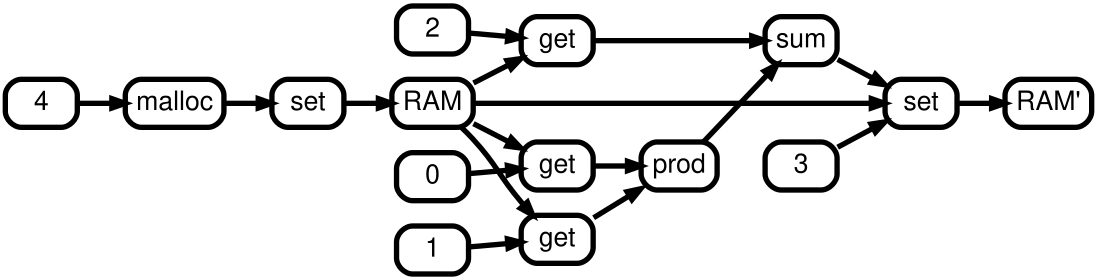
\includegraphics[scale=0.1]{rtd31}
%
%\subsection*{2. Vector multiplication}
%
%\begin{lstlisting}
%A = malloc(4);
%B = malloc(4);
%C = malloc(4);
%C[0] = A[0] * B[0];
%C[1] = A[1] * B[1];
%C[2] = A[2] * B[2];
%C[3] = A[3] * B[3];
%\end{lstlisting}
%
%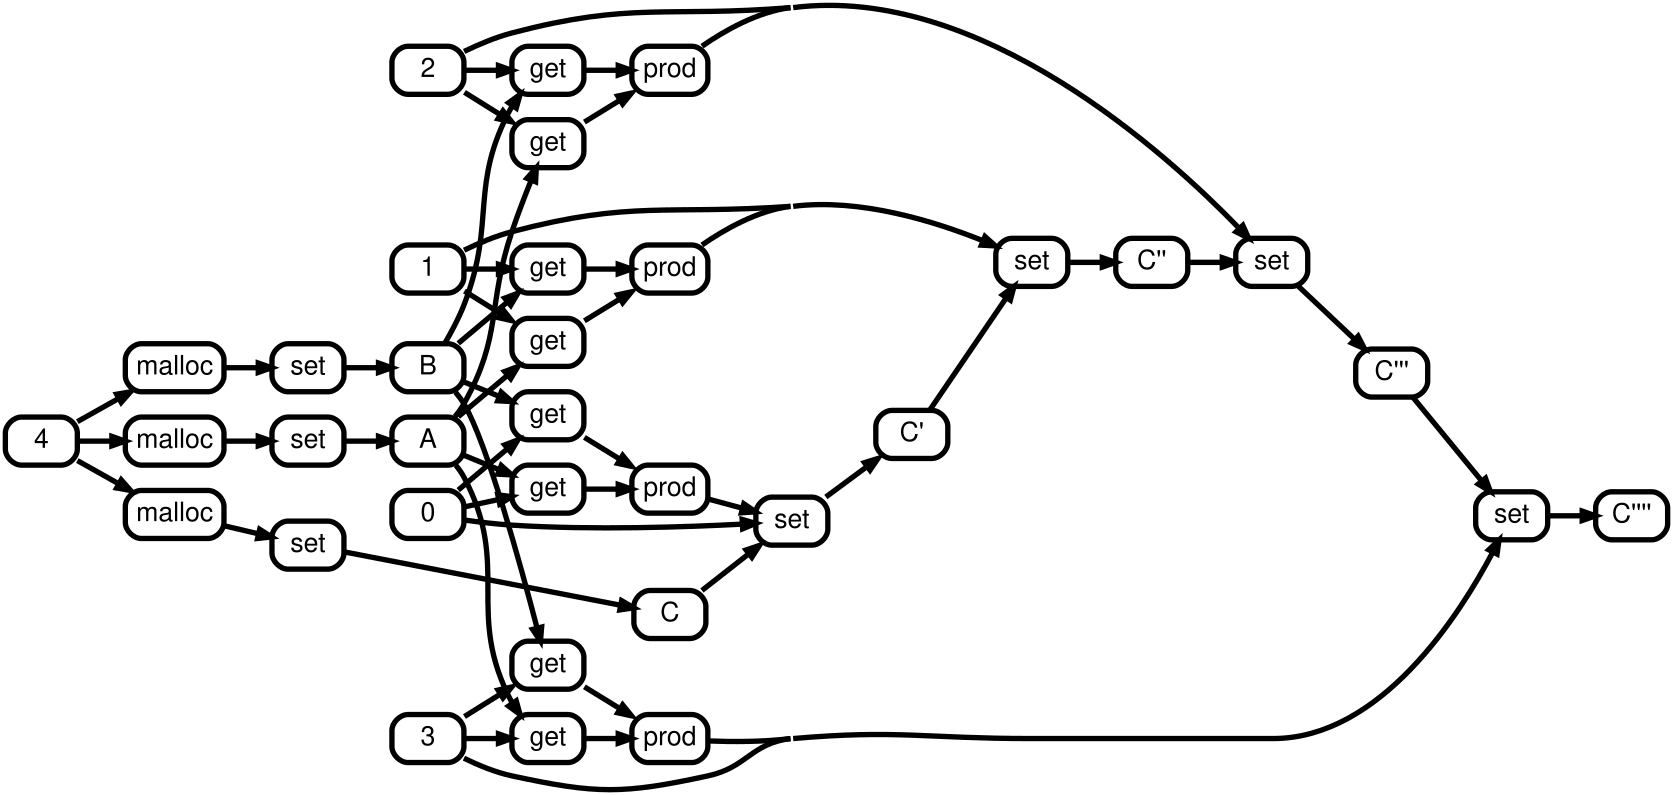
\includegraphics[scale=0.1]{rtd32}
%
%\subsection*{3. Dot product}
%
%\begin{lstlisting}
%A = malloc(4);
%B = malloc(4);
%C = malloc(1);
%C[0] = A[0] * B[0] +
%       A[1] * B[1] +
%       A[2] * B[2] +
%       A[3] * B[3];
%\end{lstlisting}
%
%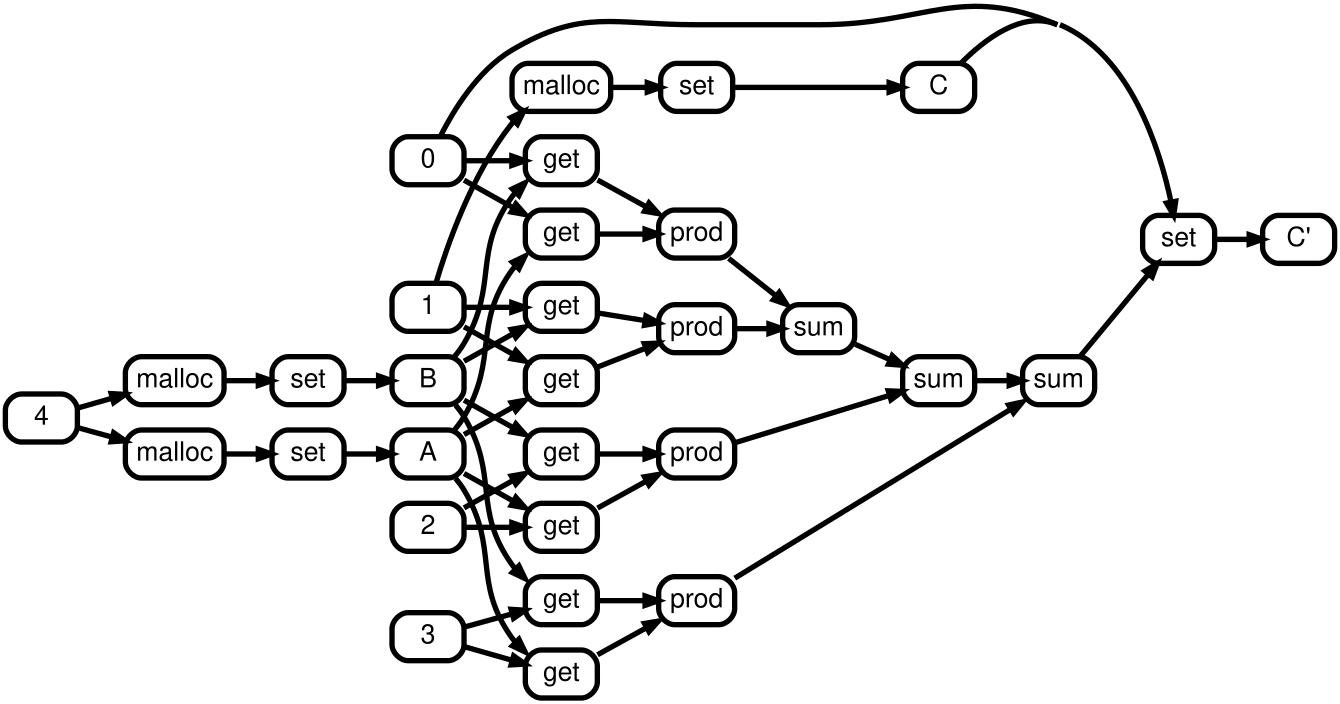
\includegraphics[scale=0.1]{rtd33}
%
%\subsection*{4. Convolution}
%
%\begin{lstlisting}
%A = malloc(6);
%W = malloc(3);
%C = malloc(4);
%C[0] = A[0] * W[0] + A[1] * W[1] + A[2] * W[2];
%C[1] = A[1] * W[0] + A[2] * W[1] + A[3] * W[2];
%C[2] = A[2] * W[0] + A[3] * W[1] + A[4] * W[2];
%C[3] = A[3] * W[0] + A[4] * W[1] + A[5] * W[2];
%\end{lstlisting}
%
%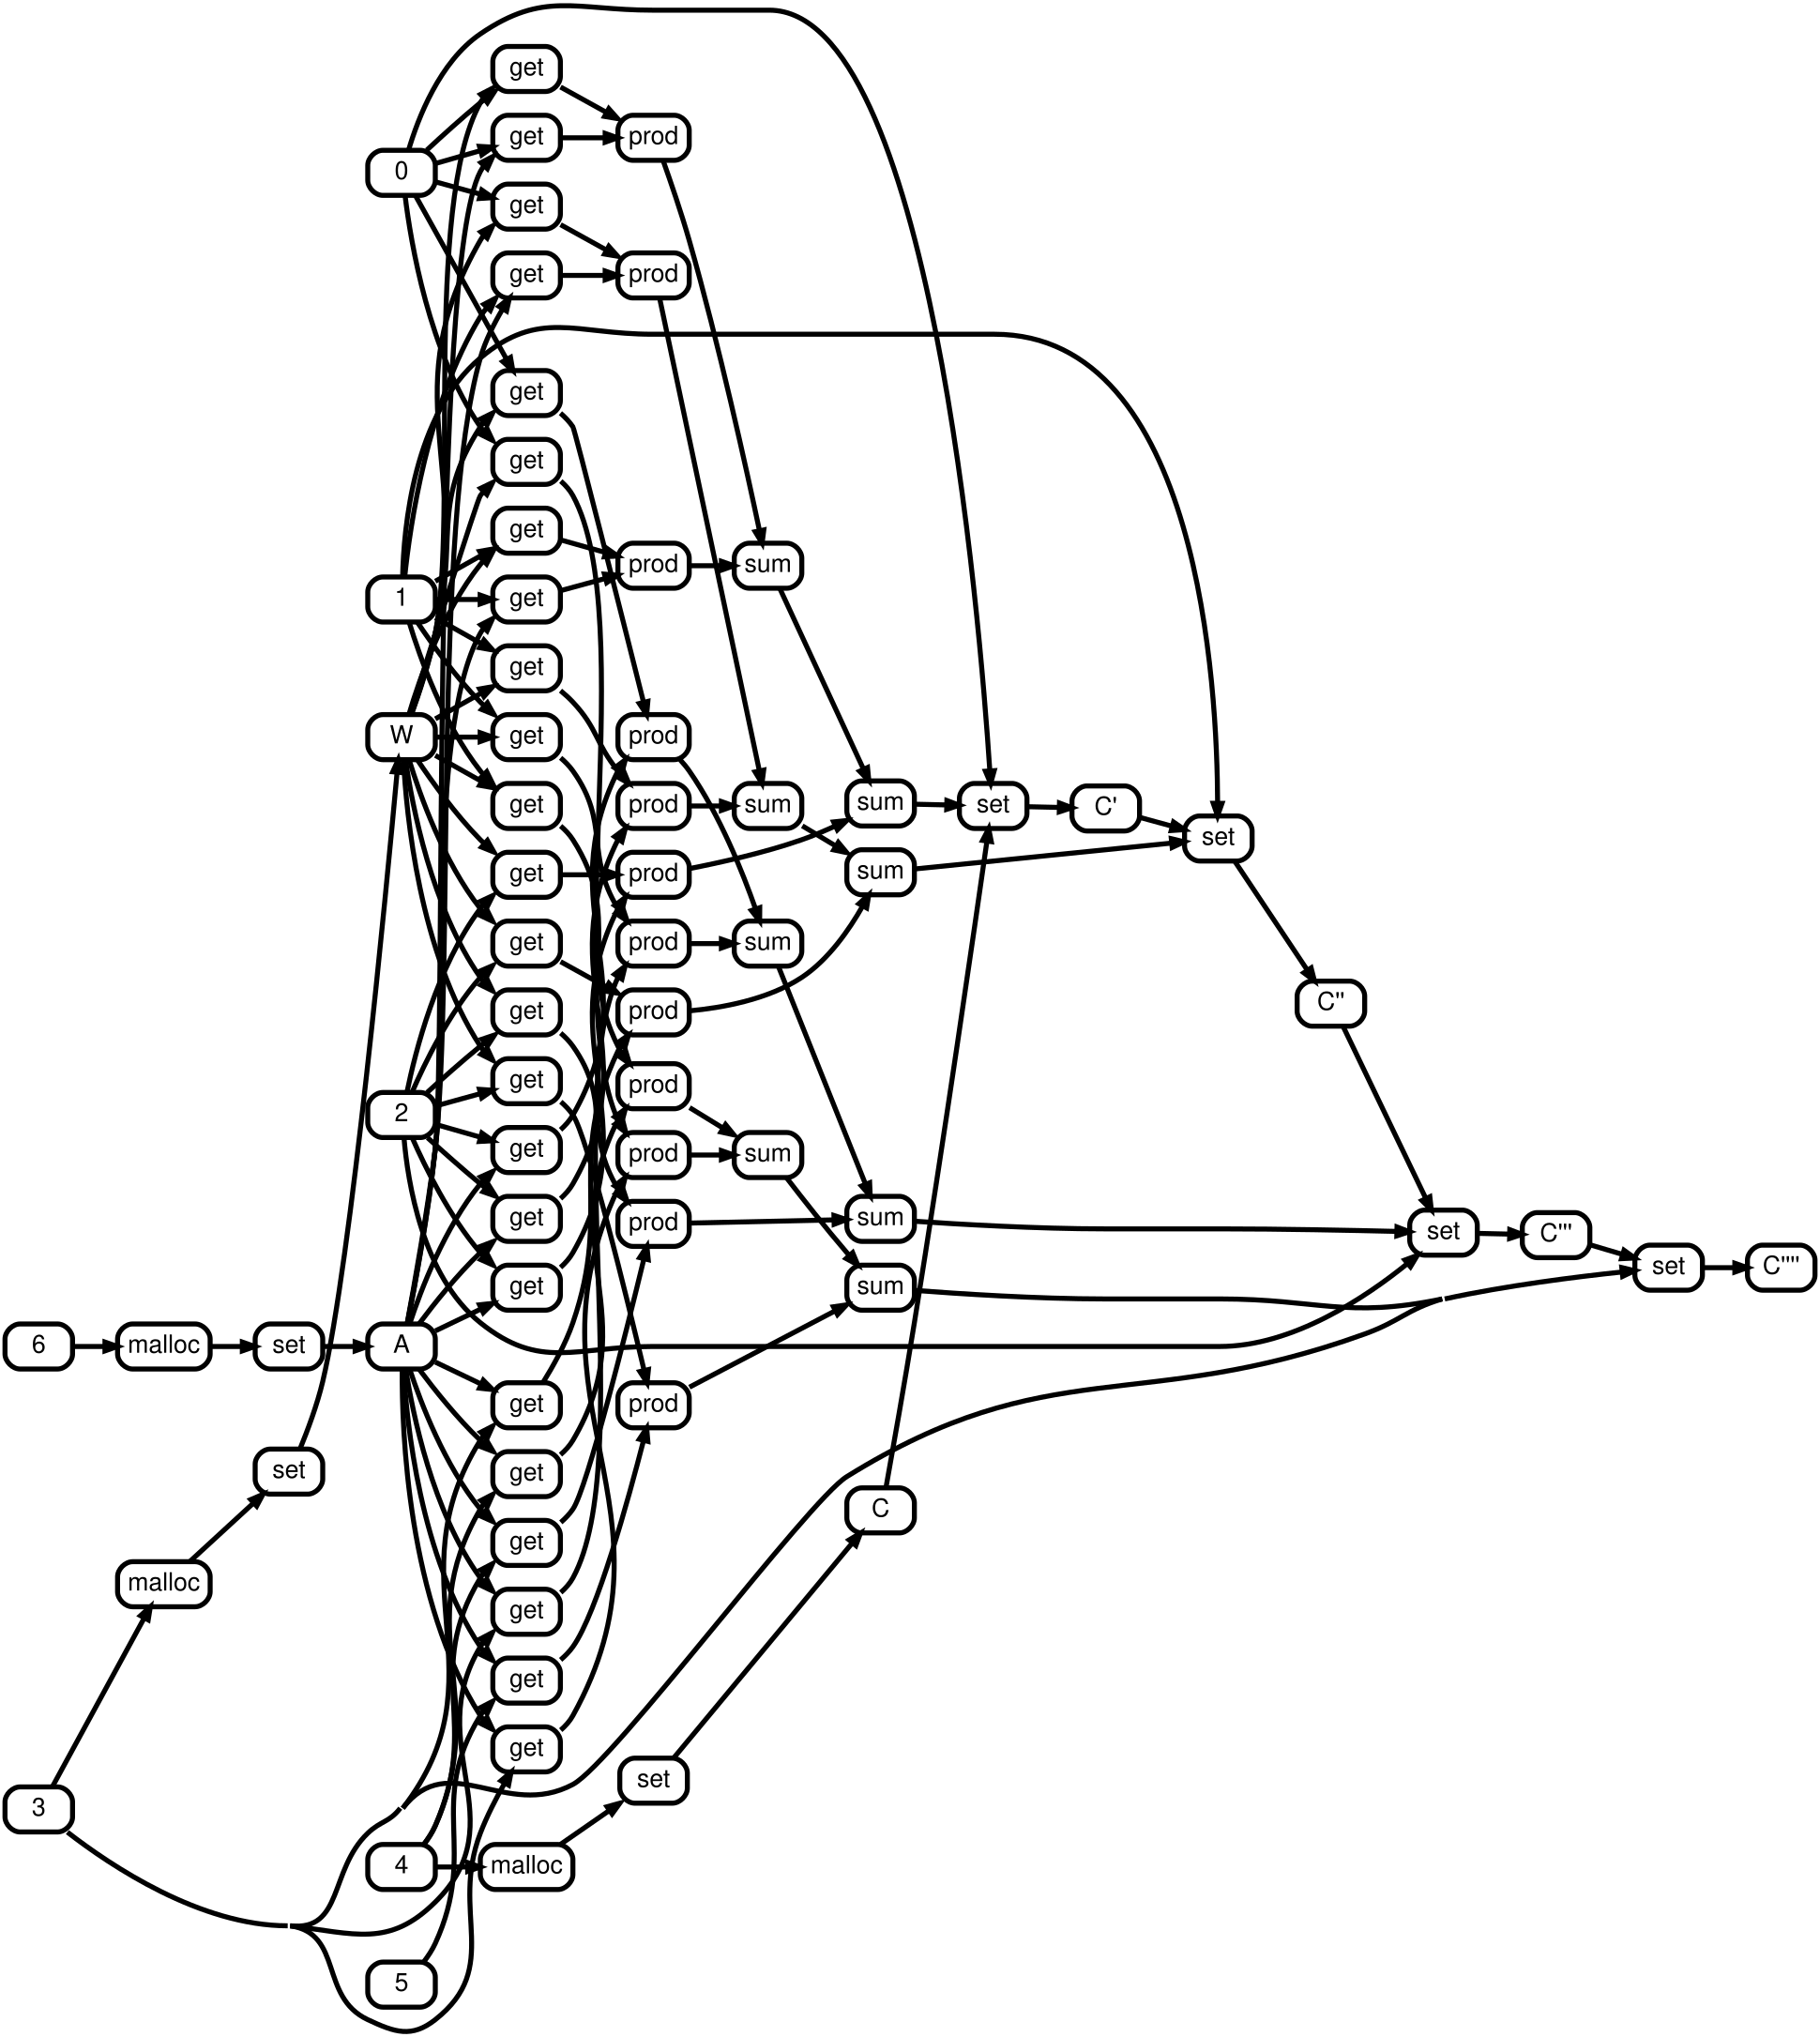
\includegraphics[scale=0.05]{rtd34}
%
%\section*{IV. Extensions/Optimizations}
%
%\subsection*{1. Simple variable test}
%
%\begin{lstlisting}
%I = 0;
%I = 1;
%I = I+J;
%\end{lstlisting}
%
%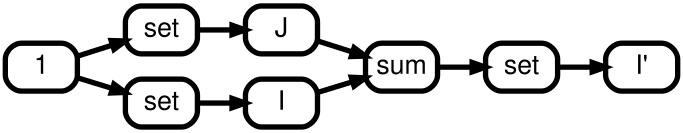
\includegraphics[scale=0.1]{rtd41}
%
%\subsection*{2. Simple loop test}
%
%\begin{lstlisting}
%S = 0.w
%for(i in 0..3) { S = S + i.w }
%\end{lstlisting}
%
%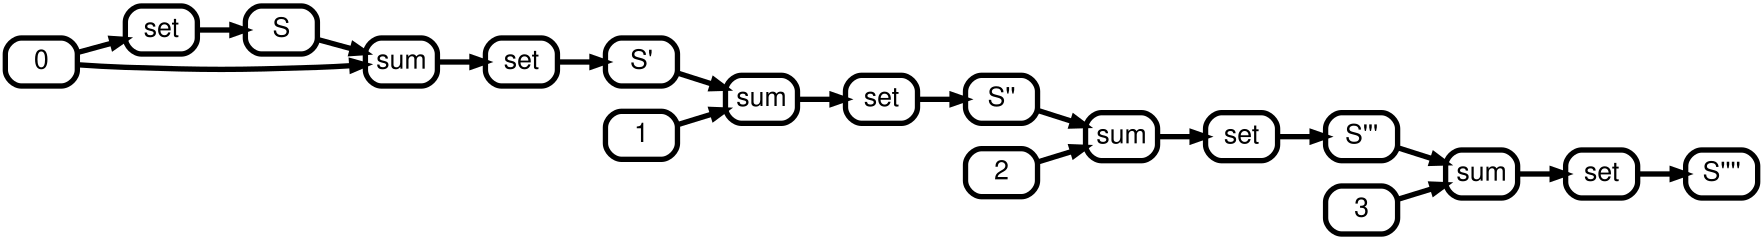
\includegraphics[scale=0.1]{rtd42}
%
%\subsection*{3. Sum of array}
%
%\begin{lstlisting}
%A = malloc(4);
%S = 0.w;
%for (i in 0..3) { S += A[i] }
%\end{lstlisting}
%
%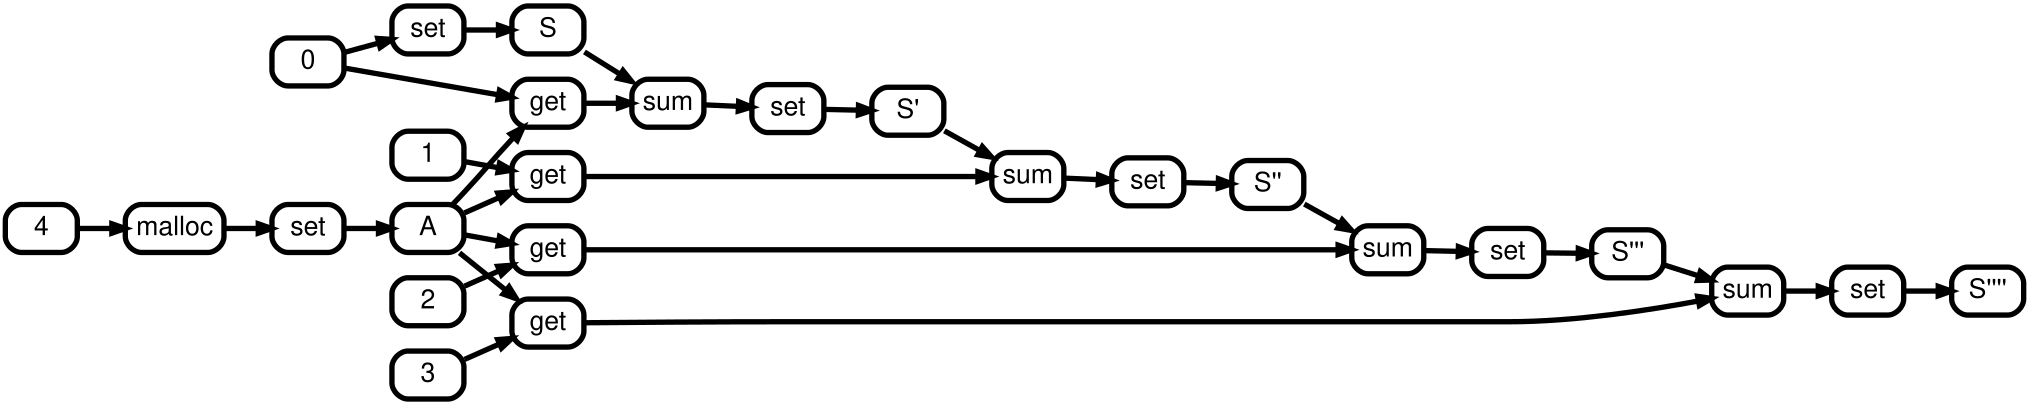
\includegraphics[scale=0.1]{rtd43}
%
%\subsection*{4. Dot product}
%
%\begin{lstlisting}
%A = malloc(4);
%B = malloc(4);
%S = 0.w;
%for (i in 0..3) { // 4 iterations
%    S = S + A[i] * B[i];
%}
%\end{lstlisting}
%
%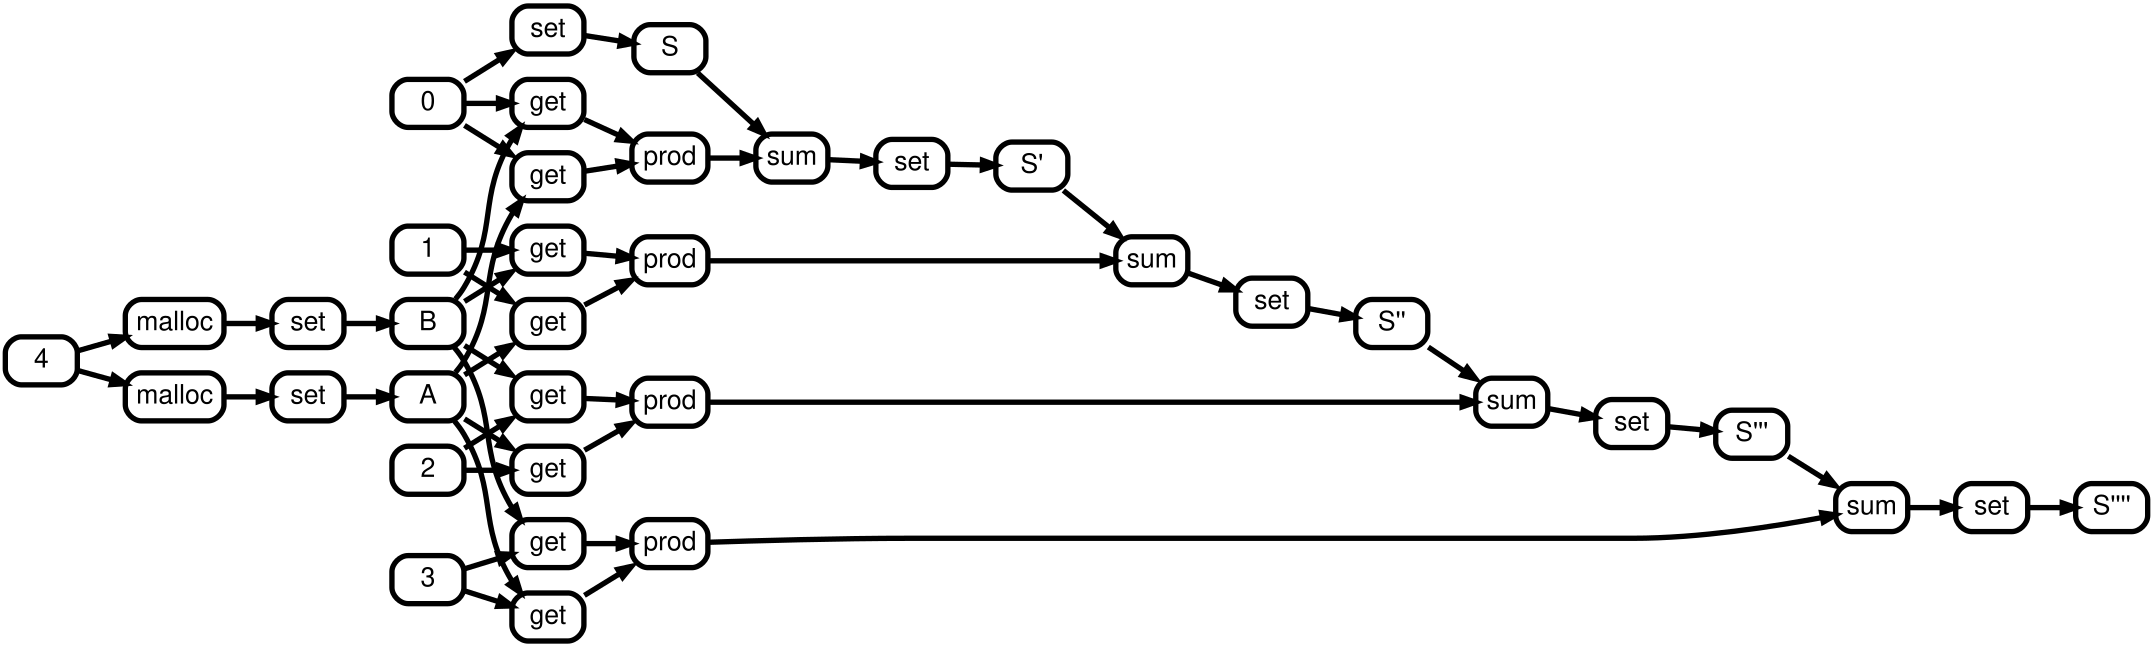
\includegraphics[scale=0.1]{rtd44}
\end{document}